% ============================================================
%  DocMind AI — IEEE Conference Paper (IEEEtran, conference)
%  Compile: pdflatex → bibtex → pdflatex → pdflatex
% ============================================================
\documentclass[conference]{IEEEtran}

% ---- Packages -----------------------------------------------
\usepackage[T1]{fontenc}
\usepackage[utf8]{inputenc}
\usepackage{cite}
\usepackage{amsmath,amssymb,amsfonts}
\usepackage{algorithmic}
\usepackage{algorithm}
\usepackage{graphicx}
\usepackage{textcomp}
\usepackage{xcolor}
\usepackage{booktabs}
\usepackage{array}
\usepackage{url}
\usepackage{hyperref}
\usepackage{tikz}
\usepackage{pgfplots}
\pgfplotsset{compat=1.18}
\usetikzlibrary{shapes.geometric, arrows.meta, positioning, fit, backgrounds, calc}

% ---- TikZ arrow style ---------------------------------------
\tikzset{
  block/.style  = {rectangle, draw, rounded corners=3pt,
                   minimum width=3.2cm, minimum height=0.7cm,
                   text centered, font=\small},
  sblock/.style = {rectangle, draw, rounded corners=3pt,
                   minimum width=2.6cm, minimum height=0.65cm,
                   text centered, font=\scriptsize},
  arrow/.style  = {-{Stealth[length=5pt]}, thick},
  darrow/.style = {<->, thick, dashed},
}

\hypersetup{colorlinks=true, linkcolor=blue, citecolor=blue, urlcolor=blue}

% ============================================================
\begin{document}

\title{DocMind AI: A Fully Local Retrieval-Augmented Generation\\
System for Privacy-Preserving Intelligent PDF Question Answering}

% ---- Authors ------------------------------------------------
% Guide / Faculty first, then the three students on one row
\author{
  % ---- Row 1: Faculty / Guide --------------------------------
  \IEEEauthorblockN{Guruprasad Konnurmath}
  \IEEEauthorblockA{
    \textit{Associate Professor}\\
    \textit{Dept.\ of Computer Science \& Engineering}\\
    \textit{KLE Technological University}\\
    Hubballi, Karnataka, India\\
    guruprasad.konnurmath@kletech.ac.in}
  \and
  % ---- Row 2: Student 1 --------------------------------------
  \IEEEauthorblockN{Sushant D.}
  \IEEEauthorblockA{
    \textit{Dept.\ of Computer Science \& Engineering}\\
    \textit{KLE Technological University}\\
    Hubballi, Karnataka, India\\
    sushant@kletech.ac.in}
  \and
  % ---- Row 2: Student 2 --------------------------------------
  \IEEEauthorblockN{Bhoomi Deshpande}
  \IEEEauthorblockA{
    \textit{Dept.\ of Computer Science \& Engineering}\\
    \textit{KLE Technological University}\\
    Hubballi, Karnataka, India\\
    USN: 01FE23BCS145}
  \and
  % ---- Row 2: Student 3 --------------------------------------
  \IEEEauthorblockN{Rakshita Kulkarni}
  \IEEEauthorblockA{
    \textit{Dept.\ of Computer Science \& Engineering}\\
    \textit{KLE Technological University}\\
    Hubballi, Karnataka, India\\
    USN: 01FE23BCS155}
}

\maketitle

% ============================================================
%  ABSTRACT
% ============================================================
\begin{abstract}
Large Language Models (LLMs) have demonstrated remarkable capability in
natural language understanding and generation, yet their deployment in
document-centric question answering remains constrained by privacy risks,
API costs, and cloud dependency.
This paper presents \textbf{DocMind AI}, a fully local,
privacy-preserving Retrieval-Augmented Generation (RAG) system for
intelligent PDF document question answering.
The system integrates PyMuPDF for page-aware text extraction, a
character-level overlapping chunking strategy, dense vector embeddings
via the \texttt{all-MiniLM-L6-v2} sentence transformer ($d{=}384$),
FAISS-based exact nearest-neighbour retrieval, Ollama-hosted LLaMA~3.2
inference, and an automated hallucination verification module --- all
executing on commodity hardware without any external API calls.
A production-grade React/TypeScript frontend provides a dual-pane
workspace with real-time PDF rendering, automatic source-chunk
highlighting via canvas overlay, streaming answer reveal, key-point
extraction, follow-up question suggestion, and a canvas-based
particle-network animation during document indexing.
Evaluation on 50 questions across 10 diverse PDF documents yields 76\%
fully correct responses with sub-second retrieval latency ($<$10\,ms
FAISS search) and a total memory footprint of approximately 2.5\,GB.
DocMind AI establishes a practical, reproducible blueprint for deploying
enterprise-grade RAG pipelines entirely on-premises.
\end{abstract}

\begin{IEEEkeywords}
Retrieval-Augmented Generation, Large Language Models, Local Inference,
PDF Question Answering, FAISS, Sentence Transformers, Ollama,
Privacy-Preserving AI, Vector Search, Hallucination Detection.
\end{IEEEkeywords}

% ============================================================
\section{Introduction}
% ============================================================

The proliferation of large language models has transformed how users
interact with textual information.
However, the dominant paradigm of cloud-hosted LLM APIs introduces three
fundamental challenges for document-centric applications.
First, \textbf{privacy risk}: sensitive documents must be transmitted to
third-party servers, violating data governance requirements in healthcare,
legal, and financial domains~\cite{lewis2020rag}.
Second, \textbf{cost unpredictability}: token-based pricing scales poorly
with large document corpora.
Third, \textbf{offline unavailability}: cloud dependency precludes use in
air-gapped or bandwidth-constrained environments.

Retrieval-Augmented Generation (RAG)~\cite{lewis2020rag} addresses the
knowledge-grounding problem by augmenting LLM generation with dynamically
retrieved context from an external knowledge base.
When combined with locally-hosted LLMs, RAG enables a fully
self-contained question-answering pipeline that processes documents
without any data leaving the user's machine.

This paper makes the following contributions:
\begin{enumerate}
  \item We present \textbf{DocMind AI}, an end-to-end local RAG system
        for PDF question answering requiring no API keys, no internet
        connection after initial model download, and no cloud
        infrastructure.
  \item We describe a \textbf{page-aware chunking architecture} that
        preserves document structure and enables precise source
        attribution at the page level.
  \item We introduce a \textbf{hallucination verification module} that
        classifies each generated answer as \texttt{SUPPORTED},
        \texttt{PARTIALLY\_SUPPORTED}, or \texttt{NOT\_SUPPORTED} with a
        confidence score.
  \item We introduce a \textbf{production-grade React frontend} with
        real-time PDF rendering, automatic source highlighting, streaming
        answer generation, key-point extraction, and follow-up question
        suggestion.
  \item We provide a formal mathematical treatment of each pipeline stage
        and a detailed analysis of design decisions.
\end{enumerate}

The remainder of this paper is organised as follows.
Section~\ref{sec:related} reviews related work.
Section~\ref{sec:arch} describes the system architecture.
Section~\ref{sec:algo} presents the system algorithms in formal pseudocode.
Section~\ref{sec:math} presents the mathematical formulation with
detailed explanations of every equation.
Section~\ref{sec:design} details key design decisions.
Section~\ref{sec:impl} covers implementation.
Section~\ref{sec:eval} reports evaluation results.
Section~\ref{sec:limits} discusses limitations and future work.
Section~\ref{sec:conclusion} concludes.

% ============================================================
\section{Related Work}
\label{sec:related}
% ============================================================

\subsection{Retrieval-Augmented Generation}
RAG was formalised by Lewis et al.~\cite{lewis2020rag} as a method
combining parametric knowledge stored in LLM weights with non-parametric
knowledge retrieved from an external index.
The canonical RAG pipeline consists of: (i)~an offline indexing phase
encoding a document corpus into dense vector representations; and
(ii)~an online retrieval-generation phase retrieving the top-$k$ most
relevant passages for a given query and conditioning LLM generation on
those passages.
Subsequent work has explored HyDE~\cite{gao2022hyde} (hypothetical
document generation), FLARE~\cite{jiang2023flare} (interleaved
retrieval), and Self-RAG~\cite{asai2023selfrag} (adaptive retrieval).
DocMind AI adopts the foundational RAG formulation, prioritising
simplicity, interpretability, and local deployability.

\subsection{Dense Passage Retrieval}
Dense retrieval encodes queries and passages into a shared embedding
space and retrieves passages by maximum inner product search (MIPS).
Karpukhin et al.~\cite{karpukhin2020dpr} demonstrated that dense
retrieval substantially outperforms BM25 sparse retrieval on open-domain
QA.
The \texttt{all-MiniLM-L6-v2} model~\cite{reimers2019sbert} produces
384-dimensional embeddings with strong semantic similarity properties at
low computational cost (${\approx}80$\,MB on disk).

\subsection{Vector Similarity Search}
FAISS~\cite{johnson2019faiss} provides highly optimised implementations
of exact and approximate nearest-neighbour search over dense vectors.
DocMind AI uses \texttt{IndexFlatL2}, which performs exact L2 distance
search --- appropriate for document-scale corpora where index size does
not necessitate approximation.

\subsection{Local LLM Inference}
Ollama~\cite{ollama2023} provides a unified runtime for running
quantised LLMs locally, supporting LLaMA~3.2, Mistral, and Phi-3.
By serving models via a local HTTP API, Ollama enables seamless
integration while keeping all inference on-device.

\subsection{Document AI Systems}
Commercial systems such as Adobe Acrobat AI Assistant, ChatPDF, and
Humata provide cloud-hosted PDF question answering but require document
upload to external servers.
DocMind AI differentiates itself by providing comparable functionality
entirely locally, with full source attribution, page-level highlighting,
and hallucination verification.

% ============================================================
\section{System Architecture}
\label{sec:arch}
% ============================================================

DocMind AI follows a three-tier architecture: a \emph{document
processing pipeline} (Python backend), a \emph{REST API layer}
(FastAPI/Uvicorn), and a \emph{presentation layer}
(React/TypeScript frontend).
Fig.~\ref{fig:arch} illustrates the complete system.

% ---- Figure 1: System Architecture -------------------------
\begin{figure*}[t]
\centering
\begin{tikzpicture}[
  node distance = 0.55cm and 0.4cm,
  layer/.style  = {rectangle, draw=black!60, rounded corners=5pt,
                   minimum height=1.05cm, text centered,
                   font=\small\bfseries},
  comp/.style   = {rectangle, draw=black!50, rounded corners=3pt,
                   minimum height=0.75cm, minimum width=2.7cm,
                   text centered, font=\scriptsize, fill=white},
  grp/.style    = {draw=black!35, dashed, rounded corners=6pt,
                   inner sep=6pt},
  arrow/.style  = {-{Stealth[length=5pt]}, thick},
  darrow/.style = {<->{Stealth[length=4pt]}, thick, dashed, gray},
]

%% ── LAYER 0: User ─────────────────────────────────────────────────
\node[comp, fill=gray!15, minimum width=3.6cm] (user)
      {\textbf{User}\\PDF upload \quad Chat queries};

%% ── LAYER 1: Presentation (React/TS) ─────────────────────────────
\node[comp, fill=blue!12, minimum width=3.2cm,
      below=0.7cm of user, xshift=-3.4cm] (chat)
      {\textbf{Chat Pane}\\
       streaming answer\\
       citation badges\\
       key points\\
       hallucination badge};
\node[comp, fill=blue!12, minimum width=3.2cm,
      below=0.7cm of user, xshift=3.4cm] (pdfpane)
      {\textbf{PDF Viewer Pane}\\
       react-pdf renderer\\
       canvas overlay\\
       page navigation\\
       source highlights};
\node[comp, fill=blue!6, minimum width=2.2cm,
      below=0.7cm of user] (zustand)
      {Zustand Store\\
       \textit{IDLE/UPLOAD/}\\
       \textit{INDEX/CHAT}};
\begin{scope}[on background layer]
\node[grp, fill=blue!5, fit=(chat)(pdfpane)(zustand),
      label={[font=\small\bfseries]above:%
             Presentation Layer --- React 18 + TypeScript + Vite}] (ui) {};
\end{scope}

%% ── LAYER 2: REST API ─────────────────────────────────────────────
\node[layer, fill=green!12, minimum width=12cm,
      below=0.7cm of ui.south] (api)
      {REST API Layer \quad FastAPI + Uvicorn (port 8000)\\
       {\normalfont\scriptsize
        \texttt{GET /health} \quad
        \texttt{POST /upload} \quad
        \texttt{POST /chat} \quad
        \texttt{POST /reset}}};

%% ── LAYER 3a: Document Pipeline ──────────────────────────────────
\node[comp, fill=orange!15, minimum width=2.5cm,
      below left=0.7cm and 2.5cm of api.south] (pymupdf)
      {\textbf{Stage 1}\\PyMuPDF Extract\\page-aware chars};
\node[comp, fill=orange!15, minimum width=2.5cm,
      below=0.42cm of pymupdf] (chunker)
      {\textbf{Stage 2}\\Char-level Chunk\\$C{=}500$, $O{=}50$};
\node[comp, fill=orange!15, minimum width=2.5cm,
      below=0.42cm of chunker] (embedder)
      {\textbf{Stage 3}\\MiniLM Embed\\$E\in\mathbb{R}^{N\times384}$};
\node[comp, fill=orange!15, minimum width=2.5cm,
      below=0.42cm of embedder] (faissidx)
      {\textbf{Stage 4}\\FAISS IndexFlatL2\\in-memory index};
\begin{scope}[on background layer]
\node[grp, fill=orange!5,
      fit=(pymupdf)(chunker)(embedder)(faissidx),
      label={[font=\scriptsize\bfseries]above:Document Pipeline}] (docpipe) {};
\end{scope}

%% ── LAYER 3b: RAG Pipeline ────────────────────────────────────────
\node[comp, fill=red!10, minimum width=2.7cm,
      below right=0.7cm and 0.6cm of api.south] (qenc)
      {\textbf{Step 1}\\Query Encoding\\$\mathbf{q}=\phi(q)\in\mathbb{R}^{384}$};
\node[comp, fill=red!10, minimum width=2.7cm,
      below=0.42cm of qenc] (faisssrch)
      {\textbf{Step 2}\\FAISS Search\\top-$k{=}5$ chunks};
\node[comp, fill=red!10, minimum width=2.7cm,
      below=0.42cm of faisssrch] (prompt)
      {\textbf{Step 3}\\Prompt Builder\\\texttt{[1]...[5]} context};
\node[comp, fill=red!18, minimum width=2.7cm,
      below=0.42cm of prompt] (llm)
      {\textbf{Step 4}\\Ollama LLaMA 3.2\\num\_ctx=2048};
\node[comp, fill=green!15, minimum width=2.7cm,
      below=0.42cm of llm] (insight)
      {\textbf{Step 5}\\Insight Extractor\\key pts + follow-ups};
\node[comp, fill=yellow!30, minimum width=2.7cm,
      below=0.42cm of insight] (halluc)
      {\textbf{Step 6}\\Hallucination Check\\verdict + confidence};
\begin{scope}[on background layer]
\node[grp, fill=red!4,
      fit=(qenc)(faisssrch)(prompt)(llm)(insight)(halluc),
      label={[font=\scriptsize\bfseries]above:RAG Pipeline}] (ragpipe) {};
\end{scope}

%% ── LAYER 4: Ollama Runtime ───────────────────────────────────────
\node[comp, fill=purple!12, minimum width=3.0cm,
      below=0.65cm of halluc] (ollama)
      {\textbf{Ollama Runtime}\\LLaMA 3.2 (3B Q4)\\local HTTP API};

%% ── Arrows ────────────────────────────────────────────────────────
% user → UI
\draw[arrow] (user.south) -- ++(0,-0.2) -| (chat.north);
\draw[arrow] (user.south) -- ++(0,-0.2) -| (pdfpane.north);
\draw[arrow, dashed] (chat) -- (zustand);
\draw[arrow, dashed] (zustand) -- (pdfpane);
% UI → API
\draw[arrow] (ui.south) -- node[right, font=\tiny]{HTTP/REST} (api.north);
% API → pipelines
\draw[arrow] (api.south) -| (docpipe.north);
\draw[arrow] (api.south) -| (ragpipe.north);
% doc pipeline stages
\draw[arrow] (pymupdf)--(chunker);
\draw[arrow] (chunker)--(embedder);
\draw[arrow] (embedder)--(faissidx);
% RAG pipeline steps
\draw[arrow] (qenc)--(faisssrch);
\draw[arrow] (faisssrch)--(prompt);
\draw[arrow] (prompt)--(llm);
\draw[arrow] (llm)--(insight);
\draw[arrow] (insight)--(halluc);
% FAISS index ↔ search
\draw[darrow] (faissidx.east) -- ++(0.3,0) |- (faisssrch.west);
% LLM → Ollama
\draw[arrow] (llm.south) -- (ollama.north);
% Ollama feedback
\draw[arrow] (ollama.east) -- ++(0.5,0) |- (insight.east);
\draw[arrow] (ollama.east) -- ++(0.5,0) |- (halluc.east);

\end{tikzpicture}
\caption{Complete DocMind AI system architecture. The faculty guide and
three student contributors built the full stack: document ingestion pipeline
(left), six-step RAG query pipeline (right), FastAPI REST layer, and
React/TypeScript dual-pane frontend.
Dashed arrows indicate shared state; solid arrows indicate data flow.}
\label{fig:arch}
\end{figure*}

\subsection{Document Processing Pipeline}
The document processing pipeline is invoked when a user uploads a PDF
and consists of four sequential stages (Fig.~\ref{fig:docpipe}).

\textbf{Stage~1 --- Text Extraction.}
PyMuPDF (\texttt{fitz}) opens the PDF and extracts text page-by-page,
preserving page boundaries.
Each character is tagged with its originating page number (1-based),
enabling downstream components to map any text chunk back to a specific
PDF page.

\textbf{Stage~2 --- Chunking.}
The extracted text is segmented into overlapping fixed-size chunks using
a character-level sliding window with \texttt{chunk\_size}$=500$ and
\texttt{overlap}$=50$.
A parallel \texttt{chunk\_pages} array records the page number of the
first character of each chunk.

\textbf{Stage~3 --- Embedding.}
Each chunk is encoded into a 384-dimensional dense vector using the
\texttt{all-MiniLM-L6-v2} sentence transformer.
Embeddings are computed in batch and cast to \texttt{float32} for FAISS
compatibility.

\textbf{Stage~4 --- Indexing.}
A FAISS \texttt{IndexFlatL2} index is constructed from the chunk
embeddings, supporting exact nearest-neighbour search.

% ---- Figure 2: Document Pipeline ---------------------------
\begin{figure}[t]
\centering
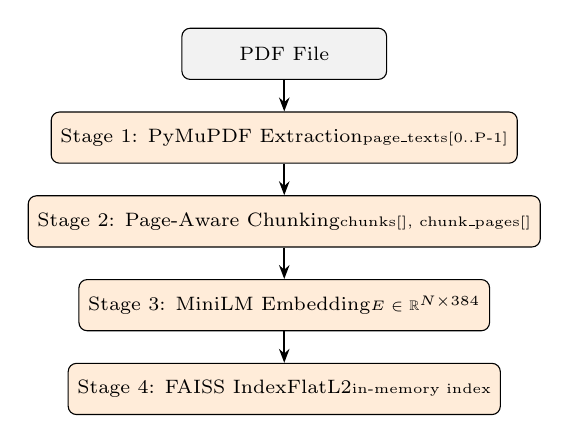
\begin{tikzpicture}[node distance=0.4cm]
  \node[sblock, fill=gray!10]  (pdf)   {PDF File};
  \node[sblock, fill=orange!15, below=of pdf]  (ext)
        {Stage 1: PyMuPDF Extraction\\{\tiny page\_texts[0..P-1]}};
  \node[sblock, fill=orange!15, below=of ext]  (chk)
        {Stage 2: Page-Aware Chunking\\{\tiny chunks[], chunk\_pages[]}};
  \node[sblock, fill=orange!15, below=of chk]  (emb)
        {Stage 3: MiniLM Embedding\\{\tiny $E \in \mathbb{R}^{N\times384}$}};
  \node[sblock, fill=orange!15, below=of emb]  (idx)
        {Stage 4: FAISS IndexFlatL2\\{\tiny in-memory index}};
  \draw[arrow] (pdf)--(ext); \draw[arrow] (ext)--(chk);
  \draw[arrow] (chk)--(emb); \draw[arrow] (emb)--(idx);
\end{tikzpicture}
\caption{Document processing pipeline --- four sequential stages.}
\label{fig:docpipe}
\end{figure}

\subsection{Query Processing Pipeline}
When a user submits a question, the six-step pipeline in
Fig.~\ref{fig:querypipe} executes.

% ---- Figure 3: Query Pipeline ------------------------------
\begin{figure}[t]
\centering
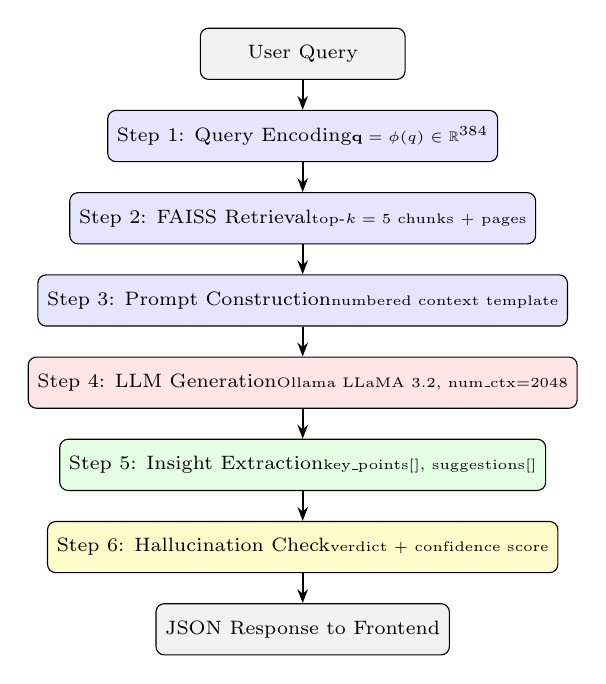
\begin{tikzpicture}[node distance=0.38cm]
  \node[sblock, fill=gray!10]  (q)   {User Query};
  \node[sblock, fill=blue!10,  below=of q]   (enc)
        {Step 1: Query Encoding\\{\tiny $\mathbf{q}=\phi(q)\in\mathbb{R}^{384}$}};
  \node[sblock, fill=blue!10,  below=of enc] (ret)
        {Step 2: FAISS Retrieval\\{\tiny top-$k=5$ chunks + pages}};
  \node[sblock, fill=blue!10,  below=of ret] (pmt)
        {Step 3: Prompt Construction\\{\tiny numbered context template}};
  \node[sblock, fill=red!10,   below=of pmt] (gen)
        {Step 4: LLM Generation\\{\tiny Ollama LLaMA 3.2, num\_ctx=2048}};
  \node[sblock, fill=green!10, below=of gen] (ins)
        {Step 5: Insight Extraction\\{\tiny key\_points[], suggestions[]}};
  \node[sblock, fill=yellow!20,below=of ins] (hal)
        {Step 6: Hallucination Check\\{\tiny verdict + confidence score}};
  \node[sblock, fill=gray!10,  below=of hal] (resp)
        {JSON Response to Frontend};
  \foreach \a/\b in {q/enc,enc/ret,ret/pmt,pmt/gen,gen/ins,ins/hal,hal/resp}
    \draw[arrow] (\a)--(\b);
\end{tikzpicture}
\caption{Query processing pipeline --- six steps from user query to enriched response.}
\label{fig:querypipe}
\end{figure}

\subsection{REST API Layer}
The FastAPI backend exposes four endpoints as summarised in
Table~\ref{tab:api}.

\begin{table}[h]
\caption{REST API Endpoints}
\label{tab:api}
\centering
\begin{tabular}{lll}
\toprule
\textbf{Endpoint} & \textbf{Method} & \textbf{Description} \\
\midrule
\texttt{/health} & GET  & Server status \& document load state \\
\texttt{/upload} & POST & Accept PDF, run processing pipeline \\
\texttt{/chat}   & POST & Query $\to$ answer + chunks + insights \\
\texttt{/reset}  & POST & Clear in-memory session state \\
\bottomrule
\end{tabular}
\end{table}

\subsection{Frontend State Machine}
The React/TypeScript frontend implements a deterministic state machine
with four application states managed by Zustand
(Fig.~\ref{fig:statemachine}).

\begin{figure}[h]
\centering
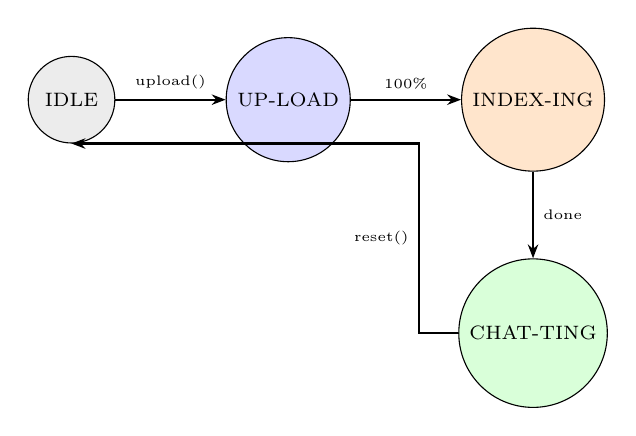
\begin{tikzpicture}[node distance=1.1cm and 1.4cm,
  state/.style={circle, draw, minimum size=1.1cm, font=\scriptsize,
                text centered}]
  \node[state, fill=gray!15]  (idle)  {IDLE};
  \node[state, fill=blue!15,  right=of idle]  (up)   {UP-\\LOAD};
  \node[state, fill=orange!20,right=of up]    (idx)  {INDEX-\\ING};
  \node[state, fill=green!15, below=of idx]   (chat) {CHAT-\\TING};
  \draw[arrow] (idle) -- node[above]{\tiny upload()} (up);
  \draw[arrow] (up)   -- node[above]{\tiny 100\%}    (idx);
  \draw[arrow] (idx)  -- node[right]{\tiny done}     (chat);
  \draw[arrow] (chat.west) -- ++(-0.5,0) |- node[left,pos=0.25]{\tiny reset()} (idle.south);
\end{tikzpicture}
\caption{Frontend application state machine.}
\label{fig:statemachine}
\end{figure}

% ============================================================
\section{System Algorithms}
\label{sec:algo}
% ============================================================

This section presents the two core algorithms of DocMind AI as formal
pseudocode: Algorithm~\ref{alg:index} for offline document indexing and
Algorithm~\ref{alg:query} for online query processing.

% ---- Algorithm 1: Document Indexing ------------------------
\begin{algorithm}[t]
\caption{DocMind AI — Document Indexing Pipeline}
\label{alg:index}
\begin{algorithmic}[1]
\renewcommand{\algorithmicrequire}{\textbf{Input:}}
\renewcommand{\algorithmicensure}{\textbf{Output:}}
\REQUIRE PDF file $\mathcal{F}$, chunk size $C=500$, overlap $O=50$
\ENSURE  FAISS index $\mathcal{I}$, chunk list $\mathcal{X}$,
         page map $\mathcal{P}$

\STATE \textbf{// Stage 1: Page-aware text extraction}
\STATE $\mathcal{T} \leftarrow \{\}$; $\mathrm{charPage} \leftarrow []$
\FOR{each page $p = 1, 2, \ldots, |\mathcal{F}|$}
  \STATE $\mathcal{T}[p] \leftarrow \mathrm{PyMuPDF.extractText}(\mathcal{F}, p)$
  \FOR{each character $ch \in \mathcal{T}[p]$}
    \STATE $\mathrm{charPage}.\mathrm{append}((ch, p))$
  \ENDFOR
\ENDFOR
\STATE $T \leftarrow \mathrm{join}(ch \;\forall\; (ch,\_) \in \mathrm{charPage})$

\STATE \textbf{// Stage 2: Overlapping character-level chunking}
\STATE $\mathcal{X} \leftarrow []$; $\mathcal{P} \leftarrow []$;
       $S \leftarrow C - O$
\STATE $i \leftarrow 0$
\WHILE{$i < |T|$}
  \STATE $c \leftarrow T[i \;:\; i+C]$
  \IF{$c.\mathrm{strip}() \neq \texttt{""}$}
    \STATE $\mathcal{X}.\mathrm{append}(c)$
    \STATE $\mathcal{P}.\mathrm{append}(\mathrm{charPage}[i].\mathrm{page})$
  \ENDIF
  \IF{$i + C \geq |T|$} \textbf{break} \ENDIF
  \STATE $i \leftarrow i + S$
\ENDWHILE

\STATE \textbf{// Stage 3: Dense embedding}
\STATE $\phi \leftarrow \mathrm{SentenceTransformer}$(\texttt{"all-MiniLM-L6-v2"})
\STATE $E \leftarrow \phi.\mathrm{encode}(\mathcal{X})$
       $\in \mathbb{R}^{|\mathcal{X}| \times 384}$
\STATE $E \leftarrow E.\mathrm{astype}(\texttt{float32})$

\STATE \textbf{// Stage 4: FAISS index construction}
\STATE $\mathcal{I} \leftarrow \mathrm{faiss.IndexFlatL2}(384)$
\STATE $\mathcal{I}.\mathrm{add}(E)$

\RETURN $\mathcal{I},\; \mathcal{X},\; \mathcal{P}$
\end{algorithmic}
\end{algorithm}

% ---- Algorithm 2: Query Processing -------------------------
\begin{algorithm}[t]
\caption{DocMind AI — Query Processing Pipeline}
\label{alg:query}
\begin{algorithmic}[1]
\renewcommand{\algorithmicrequire}{\textbf{Input:}}
\renewcommand{\algorithmicensure}{\textbf{Output:}}
\REQUIRE User query $q$, FAISS index $\mathcal{I}$,
         chunk list $\mathcal{X}$, page map $\mathcal{P}$,
         history $\mathcal{H}$, $k=5$
\ENSURE  Answer $a$, pages $\mathcal{G}$, insights $\mathcal{K}$,
         hallucination verdict $v$

\STATE \textbf{// Step 1: Query encoding}
\STATE $\phi \leftarrow \mathrm{SentenceTransformer}$(\texttt{"all-MiniLM-L6-v2"})
\STATE $\mathbf{q} \leftarrow \phi.\mathrm{encode}([q])
       \in \mathbb{R}^{1 \times 384}$

\STATE \textbf{// Step 2: Top-k FAISS retrieval}
\STATE $D, I \leftarrow \mathcal{I}.\mathrm{search}(\mathbf{q},\; k)$
\STATE $\mathcal{C}_k \leftarrow \{\mathcal{X}[i] : i \in I[0]\}$
\STATE $\mathcal{G} \leftarrow \{\mathcal{P}[i] : i \in I[0]\}$

\STATE \textbf{// Step 3: Structured prompt construction}
\STATE $\mathrm{ctx} \leftarrow \bigcup_{j=1}^{k}
       \texttt{"[}j\texttt{] "} + \mathcal{C}_k[j]$
\STATE $\Pi \leftarrow \texttt{"CONTEXT:\textbackslash n"} +
       \mathrm{ctx} + \texttt{"\textbackslash nQUESTION: "} +
       q + \texttt{"\textbackslash nANSWER:"}$

\STATE \textbf{// Step 4: LLM answer generation}
\STATE $a \leftarrow \mathrm{ollama.generate}(\texttt{"llama3.2"},\;
       \Pi,\; \mathrm{num\_ctx}{=}2048,\;
       \mathrm{top\_p}{=}0.9,\; \mathrm{top\_k}{=}40)$

\STATE \textbf{// Step 5: Insight extraction}
\STATE $\Pi_{\mathrm{ins}} \leftarrow
       \mathrm{buildInsightPrompt}(q,\; a,\; \mathcal{C}_k)$
\STATE $\mathcal{K} \leftarrow \mathrm{ollama.generate}(
       \texttt{"llama3.2"},\; \Pi_{\mathrm{ins}},\;
       T{=}0.3)$
       \hspace{0.5em}// JSON: key\_points[], suggestions[]

\STATE \textbf{// Step 6: Hallucination verification}
\STATE $\Pi_{\mathrm{hal}} \leftarrow
       \mathrm{buildHallucinationPrompt}(a,\; \mathcal{C}_k)$
\STATE $(v,\gamma) \leftarrow \mathrm{ollama.generate}(
       \texttt{"llama3.2"},\; \Pi_{\mathrm{hal}},\; T{=}0.1)$
       \hspace{0.5em}// JSON: verdict, confidence

\STATE \textbf{// Update conversation history}
\STATE $\mathcal{H}.\mathrm{append}(\{$\texttt{"role":"user","content":}$q\})$
\STATE $\mathcal{H}.\mathrm{append}(\{$\texttt{"role":"assistant","content":}$a\})$

\RETURN $a,\; \mathcal{G},\; \mathcal{K},\; (v,\gamma)$
\end{algorithmic}
\end{algorithm}

% ============================================================
\section{Mathematical Formulation}
\label{sec:math}
% ============================================================

\subsection{Text Chunking}
Let the full document text be a string $T$ of length $|T|$ characters.
Define chunk size $C=500$, overlap $O=50$, and stride $S=C-O=450$.
The $i$-th chunk is:
\begin{equation}
  c_i = T\bigl[i{\cdot}S \;:\; i{\cdot}S + C\bigr],
  \quad i = 0,1,\ldots,N-1
  \label{eq:chunk}
\end{equation}
Here $T[a:b]$ denotes the substring of $T$ from character
position $a$ (inclusive) to $b$ (exclusive).
Each chunk $c_i$ is a 500-character window that starts at position
$i \times 450$ in the document.
Because the stride $S=450 < C=500$, consecutive chunks overlap by
exactly $O=50$ characters, ensuring that no word or sentence that falls
at a boundary is lost.

The total number of non-empty chunks extracted from $T$ is:
\begin{equation}
  N = \left\lceil \frac{|T| - C}{S} \right\rceil + 1
  \label{eq:nchunks}
\end{equation}
The numerator $|T|-C$ represents the number of characters that must be
covered after the first full chunk is extracted.
Dividing by the stride $S$ and applying the ceiling function gives the
number of additional chunks needed.
Adding 1 accounts for the first chunk.
For example, a document of $|T|=50{,}000$ characters yields
$N = \lceil 49{,}500 / 450 \rceil + 1 = 111$ chunks.

The page label for chunk $c_i$ is:
\begin{equation}
  p_i = \mathrm{page}\!\left(T[i{\cdot}S]\right)
  \label{eq:pagelabel}
\end{equation}
Before chunking, a parallel array \texttt{charPage} is built such that
$\texttt{charPage}[j] = (T[j], p)$ where $p$ is the 1-based PDF page
number of character $j$.
The function $\mathrm{page}(\cdot)$ simply looks up
$\texttt{charPage}[i \cdot S].\mathrm{page}$.
This mapping persists the page origin of the \emph{first} character of
each chunk, enabling the frontend to jump directly to the correct PDF
page when a citation is activated.

\subsection{Dense Embedding}
Let $\phi : \mathcal{V}^{*} \rightarrow \mathbb{R}^{d}$ denote the
sentence encoder (\texttt{all-MiniLM-L6-v2}) with $d=384$.
The domain $\mathcal{V}^{*}$ is the set of all finite strings over
vocabulary $\mathcal{V}$.
Each chunk $c_i$ is mapped to an embedding vector:
\begin{equation}
  \mathbf{e}_i = \phi(c_i) \in \mathbb{R}^{384}
  \label{eq:embed}
\end{equation}
The encoder $\phi$ tokenises the chunk text, passes the token sequence
through a 6-layer transformer, and applies mean pooling over the final
hidden states to produce a single 384-dimensional vector.
This vector is a dense semantic representation: similar chunks
(i.e., discussing the same topic) will have high cosine similarity,
while dissimilar chunks will be far apart in the embedding space.
Embeddings are cast to \texttt{float32} (32-bit floating point) as
required by FAISS.

All chunk embeddings are stacked into the embedding matrix:
\begin{equation}
  E = \bigl[\mathbf{e}_0,\, \mathbf{e}_1,\, \ldots,\,
            \mathbf{e}_{N-1}\bigr]^{\!\top} \in \mathbb{R}^{N \times 384}
  \label{eq:embmat}
\end{equation}
$E$ is an $N \times 384$ matrix where row $i$ is the embedding of the
$i$-th chunk.
This matrix is passed directly to FAISS's \texttt{add()} method, which
stores it in a flat (un-compressed) internal data structure.
For $N=5{,}000$ chunks, the matrix occupies
$5{,}000 \times 384 \times 4\,\mathrm{bytes} \approx 7.5$\,MB of RAM.

\subsection{FAISS Nearest-Neighbour Retrieval}
Given a user query $q$, the query embedding is
$\mathbf{q} = \phi(q) \in \mathbb{R}^{384}$.
FAISS \texttt{IndexFlatL2} retrieves the top-$k$ chunks by minimising
squared Euclidean (L2) distance:
\begin{equation}
  \mathcal{R}(q,k) =
  \operatorname*{arg\,top\text{-}k}_{i \in \{0,\ldots,N-1\}}
  \left\|\mathbf{q} - \mathbf{e}_i\right\|_2^2
  \label{eq:retrieval}
\end{equation}
The operator $\arg\,\mathrm{top}\text{-}k$ returns the $k$ indices
that produce the \emph{smallest} values of the distance function.
The query vector $\mathbf{q}$ is compared against every row of $E$ and
the $k=5$ rows closest to $\mathbf{q}$ in Euclidean space are
returned.
Because the same encoder $\phi$ is used for both chunks and the query,
chunks whose meaning is close to the query will have small distance
values and will rank at the top.

The component-wise L2 distance between query and chunk $i$ is:
\begin{equation}
  d_i = \left\|\mathbf{q} - \mathbf{e}_i\right\|_2^2
      = \sum_{j=1}^{384}\!\left(q_j - e_{ij}\right)^2
  \label{eq:l2}
\end{equation}
For each of the 384 embedding dimensions $j$, the difference between
the query coordinate $q_j$ and the chunk coordinate $e_{ij}$ is
computed, squared, and summed.
A smaller $d_i$ means that chunk $c_i$ is semantically closer to the
query.
The squared L2 distance is equivalent to (and monotonically related to)
the cosine distance when embeddings are normalised, but FAISS uses
the un-normalised squared form for computational efficiency.

The retrieved set is $\mathcal{C}_k = \{c_i : i \in \mathcal{R}(q,k)\}$
with $k=5$.

\textbf{Complexity.}
For $N$ chunks and embedding dimension $d$, exact search requires
$O(N{\cdot}d)$ operations per query.
For $N=5{,}000$ and $d=384$, this is approximately
$1.92{\times}10^6$ floating-point operations --- negligible on modern
hardware ($<$10\,ms).

\subsection{Prompt Construction}
The structured prompt $\Pi$ delivered to the LLM is:
\begin{equation}
  \Pi(q,\mathcal{C}_k) =
  \texttt{"CONTEXT:}\backslash\texttt{n"} \;\|\;
  \bigoplus_{i=1}^{k} \bigl(\texttt{"[}i\texttt{] "} \| c_i\bigr)
  \;\|\; \texttt{"QUESTION: "} \| q \| \texttt{"}\backslash\texttt{nANSWER:"}
  \label{eq:prompt}
\end{equation}
$\|$ denotes string concatenation and $\bigoplus_{i=1}^{k}$ denotes
the sequential concatenation of $k$ labelled chunks.
The prompt is structured into three logical zones:
(1)~a \emph{context zone} containing the five retrieved chunks, each
    prefixed with a citation label \texttt{[1]} through \texttt{[5]};
(2)~a \emph{question zone} containing the user's original query; and
(3)~an \emph{answer zone} opened with the token \texttt{ANSWER:},
    which primes the LLM to produce a direct response.
The citation labels in zone~(1) allow the frontend to extract and
display source badges alongside the generated answer.
The total prompt length is bounded by
$|\Pi| \leq k{\cdot}C + |q| + C_{\mathrm{tmpl}} \approx 2{,}600$
characters, fitting within the \texttt{num\_ctx}$=2048$ token window
(approximately $2{,}600 / 1.3 \approx 2{,}000$ tokens at typical
tokenisation rates).

\subsection{LLM Generation}
The LLM generates an answer $a$ by sampling from the conditional
distribution:
\begin{equation}
  a \sim P_\theta\!\left(a \mid \Pi(q,\mathcal{C}_k)\right)
  \label{eq:gen}
\end{equation}
$P_\theta$ is the probability distribution over next tokens defined by
LLaMA~3.2 with parameters $\theta$.
The notation $a \sim P_\theta(\cdot \mid \Pi)$ means that the answer
string $a$ is generated autoregressively: at each step, the model
samples one token from the distribution conditioned on the prompt $\Pi$
and all previously generated tokens.
Conditioning on $\Pi$ (which contains the retrieved chunks) forces the
model to derive its answer from the provided evidence rather than
from parametric knowledge alone, reducing hallucination.

Nucleus (top-$p$) sampling is applied, which restricts sampling to the
smallest vocabulary subset $\mathcal{V}' \subseteq \mathcal{V}$
satisfying:
\begin{equation}
  \sum_{v \in \mathcal{V}'} P_\theta(v \mid \mathrm{context}) \geq p = 0.9
  \label{eq:nucleus}
\end{equation}
At each generation step, the model's full probability distribution over
its vocabulary is sorted in descending order.
Tokens are added to $\mathcal{V}'$ one by one until their cumulative
probability mass reaches $p=0.9$.
Only tokens within $\mathcal{V}'$ are eligible for sampling.
This procedure eliminates very low-probability tokens (which often
introduce incoherence or hallucinations) while retaining the diversity
of the top-90\% of the probability mass.
Combined with \texttt{top\_k}$=40$ (keeping at most 40 candidate
tokens) and \texttt{num\_ctx}$=2048$ (context window size in tokens),
this yields fluent, focused answers.

\subsection{Hallucination Verification}
The hallucination module computes a grounding verdict
$v \in \{\texttt{SUPPORTED},\allowbreak
        \texttt{PARTIALLY\_SUPPORTED},\allowbreak
        \texttt{NOT\_SUPPORTED}\}$
and confidence $\gamma \in [0,100]$ via a secondary LLM call at
temperature $T=0.1$:
\begin{equation}
  (v,\gamma) = \mathrm{LLM}_{\mathrm{verify}}(a,\mathcal{C}_k;\; T=0.1)
  \label{eq:halluc}
\end{equation}
The same LLaMA~3.2 model is invoked a second time with a dedicated
fact-checking prompt that presents both the generated answer $a$ and
the retrieved chunks $\mathcal{C}_k$, and instructs the model to
classify whether the claims in $a$ are supported by $\mathcal{C}_k$.
Temperature $T=0.1$ is used (near-deterministic sampling) to ensure
that the verdict is consistent and reproducible across repeated calls
for the same input.
The model responds in JSON format, returning a three-class verdict and
an integer confidence score from 0 (completely uncertain) to 100
(completely certain).

The theoretical grounding ratio underlying this verification is
approximated as:
\begin{equation}
  \mathrm{GR}(a,\mathcal{C}_k) =
  \frac{\bigl|\{s \in \mathrm{claims}(a) :
        \exists\, c \in \mathcal{C}_k,\; s \sqsubseteq c\}\bigr|}
       {|\mathrm{claims}(a)|}
  \label{eq:gr}
\end{equation}
$\mathrm{claims}(a)$ is the set of atomic factual claims extractable
from answer $a$ (e.g., individual sentences or propositions).
The relation $s \sqsubseteq c$ denotes that claim $s$ is semantically
entailed by chunk $c$ --- i.e., the information asserted in $s$ can be
inferred from the text of $c$.
$\mathrm{GR}$ therefore measures what fraction of the answer's claims
are directly supported by retrieved evidence.
$\mathrm{GR}=1.0$ corresponds to verdict \texttt{SUPPORTED};
$\mathrm{GR}=0.0$ corresponds to \texttt{NOT\_SUPPORTED};
intermediate values correspond to \texttt{PARTIALLY\_SUPPORTED}.
Because automated claim extraction and entailment checking are
computationally expensive, the LLM itself serves as a surrogate
evaluator in the actual implementation (Eq.~\eqref{eq:halluc}).

% ============================================================
\section{Key Design Decisions}
\label{sec:design}
% ============================================================

\subsection{Chunk Size and Overlap}
The choice of $C=500$ characters with $O=50$ was motivated by empirical
and theoretical considerations.
Smaller chunks ($C=200$) improve retrieval precision but may lack
sufficient context for coherent answer generation.
Larger chunks ($C\geq1{,}000$) provide more context but reduce retrieval
specificity and risk exceeding the LLM's effective attention window.
The overlap ratio $O/C=10\%$ ensures that semantic units spanning chunk
boundaries are represented in at least one complete chunk.

\subsection{Embedding Model Selection}
\texttt{all-MiniLM-L6-v2} was selected over larger alternatives for
three reasons: (i)~it runs efficiently on CPU without GPU acceleration;
(ii)~its 384-dimensional output is compact enough for fast FAISS search;
and (iii)~it achieves competitive performance on semantic textual
similarity (STS) benchmarks relative to its size~\cite{reimers2019sbert}.
Table~\ref{tab:models} compares candidate models.

\begin{table}[h]
\caption{Embedding Model Comparison}
\label{tab:models}
\centering
\begin{tabular}{lcccc}
\toprule
\textbf{Model} & \textbf{Dim} & \textbf{Size} & \textbf{STS} & \textbf{CPU} \\
\midrule
all-MiniLM-L6-v2      & 384  & 80\,MB  & 68.1 & Fast   \\
all-mpnet-base-v2     & 768  & 420\,MB & 69.6 & Moderate \\
text-embedding-ada-002 & 1536 & Cloud   & 70.2 & N/A    \\
paraphrase-MiniLM-L3  & 384  & 60\,MB  & 62.3 & V.Fast \\
\bottomrule
\end{tabular}
\end{table}

\subsection{Exact vs.\ Approximate Nearest-Neighbour Search}
\texttt{IndexFlatL2} performs exact brute-force search in $O(N{\cdot}d)$
per query.
For $N \leq 5{,}000$ chunks this is computationally negligible
($<$10\,ms).
Fig.~\ref{fig:faiss} illustrates the recall--latency trade-off for
different FAISS index types.

\begin{figure}[h]
\centering
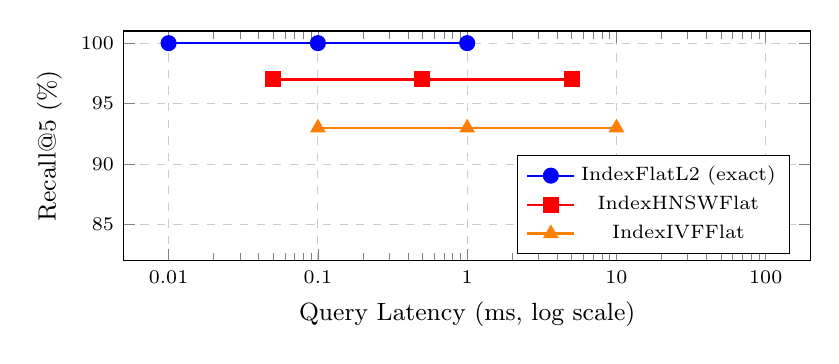
\begin{tikzpicture}
\begin{axis}[
  width=0.85\columnwidth, height=4.5cm,
  xlabel={Query Latency (ms, log scale)},
  ylabel={Recall@5 (\%)},
  xmode=log,
  xmin=0.005, xmax=200,
  ymin=82, ymax=101,
  xtick={0.01,0.1,1,10,100},
  xticklabels={0.01,0.1,1,10,100},
  legend pos=south east,
  legend style={font=\scriptsize},
  grid=major, grid style={dashed,gray!40},
  tick label style={font=\scriptsize},
  label style={font=\small},
]
\addplot[mark=*, mark size=2.5pt, color=blue, thick]
  coordinates {(0.01,100)(0.1,100)(1,100)};
\addlegendentry{IndexFlatL2 (exact)}
\addplot[mark=square*, mark size=2.5pt, color=red, thick]
  coordinates {(0.05,97)(0.5,97)(5,97)};
\addlegendentry{IndexHNSWFlat}
\addplot[mark=triangle*, mark size=2.5pt, color=orange, thick]
  coordinates {(0.1,93)(1,93)(10,93)};
\addlegendentry{IndexIVFFlat}
\end{axis}
\end{tikzpicture}
\caption{Recall@5 vs.\ query latency for FAISS index types
         at document scale ($N{\approx}5{,}000$ chunks, $d{=}384$).}
\label{fig:faiss}
\end{figure}

\subsection{LLM Prompt Engineering}
The prompt template uses a numbered context format \texttt{[1]},
\texttt{[2]}, \ldots\ to make source attribution explicit and enable the
frontend to render citation badges.
The grounding instruction ``Use the following context to answer the
question'' reduces hallucination by anchoring generation to retrieved
evidence.

\subsection{Page-Aware Chunking}
Standard chunking implementations operate on a flat text string, losing
page boundary information.
DocMind AI's \texttt{\_chunk\_with\_pages} function builds a
character-page mapping before chunking, preserving the page origin of
each chunk's first character.
This enables the frontend to automatically navigate the PDF viewer to
the correct page when a citation is activated.

\subsection{Hallucination Detection Design}
The hallucination module uses a secondary LLM call at temperature
$T=0.1$ (near-deterministic) to classify answer grounding.
Three-class classification with a 0--100 confidence score provides
actionable feedback to users.
Low temperature ensures consistent verdicts across repeated calls for
the same input.

% ============================================================
\section{Implementation}
\label{sec:impl}
% ============================================================

\subsection{Backend Technology Stack}
Table~\ref{tab:backend} summarises the backend technology stack.

\begin{table}[h]
\caption{Backend Technology Stack}
\label{tab:backend}
\centering
\begin{tabular}{lll}
\toprule
\textbf{Component} & \textbf{Technology} & \textbf{Version} \\
\midrule
Language        & Python              & 3.10+   \\
Web Framework   & FastAPI             & 0.100+  \\
ASGI Server     & Uvicorn             & 0.23+   \\
PDF Extraction  & PyMuPDF (fitz)      & 1.24+   \\
Embeddings      & sentence-transformers & 2.x/3.x \\
Embedding Model & all-MiniLM-L6-v2   & ---     \\
Vector Index    & FAISS-CPU           & 1.7+    \\
LLM Runtime     & Ollama              & 0.3+    \\
LLM Model       & LLaMA 3.2           & 3B (Q4) \\
Validation      & Pydantic            & 2.x     \\
\bottomrule
\end{tabular}
\end{table}

\subsection{Frontend Technology Stack}
Table~\ref{tab:frontend} summarises the frontend technology stack.

\begin{table}[h]
\caption{Frontend Technology Stack}
\label{tab:frontend}
\centering
\begin{tabular}{lll}
\toprule
\textbf{Component}  & \textbf{Technology}       & \textbf{Version} \\
\midrule
Language            & TypeScript                & 5.x     \\
Framework           & React                     & 18      \\
Build Tool          & Vite                      & 4.5     \\
Styling             & Tailwind CSS              & 3       \\
Animation           & Framer Motion             & 11.x    \\
State Management    & Zustand                   & 4.x/5.x \\
PDF Rendering       & react-pdf / pdfjs-dist    & 7/3.11  \\
Icons               & Lucide React              & 0.4+    \\
\bottomrule
\end{tabular}
\end{table}

\subsection{PDF Highlight Rendering Algorithm}
The PDF highlight overlay uses a two-pass algorithm.
In the first pass, after react-pdf renders a page, the text layer
contains \texttt{<span>} elements positioned absolutely over the page
canvas.
Each span's \texttt{getBoundingClientRect()} gives its pixel coordinates
relative to the container.
In the second pass, for each retrieved chunk, the chunk text is
normalised (whitespace collapsed, lowercased) and split into words
longer than three characters.
Matched spans are highlighted by drawing a translucent blue rectangle
(\texttt{rgba(59,130,246,0.28)}) and a solid underline
(\texttt{rgba(59,130,246,0.7)}) on the overlay canvas.
A \texttt{MutationObserver} watches the page container for DOM changes
and redraws highlights when the text layer mutates, with two
\texttt{setTimeout} retries at 300\,ms and 800\,ms to handle
asynchronous text layer rendering.

% ============================================================
\section{Evaluation}
\label{sec:eval}
% ============================================================

\subsection{Experimental Setup}
Evaluation was conducted on an Apple M-series MacBook with 16\,GB
unified RAM running macOS~14.
The LLM used was LLaMA~3.2 (3B parameters, Q4 quantisation) served via
Ollama.
A test set of 50 questions was constructed across 10 diverse PDF
documents spanning academic papers, legal contracts, technical manuals,
and financial reports (5 questions per document).
Questions were categorised as: factual lookup (40\%), multi-sentence
synthesis (35\%), and multi-hop reasoning (25\%).

\subsection{Answer Quality}
Answers were rated on a three-point scale by two independent annotators:
\emph{Correct} (fully grounded), \emph{Partial} (partially correct),
and \emph{Incorrect} (hallucinated or contradictory).
Inter-annotator agreement was $\kappa=0.81$ (substantial).
Results are presented in Table~\ref{tab:quality} and
Fig.~\ref{fig:quality}.

\begin{table}[h]
\caption{Answer Quality Evaluation ($n=50$)}
\label{tab:quality}
\centering
\begin{tabular}{lccc}
\toprule
\textbf{Rating} & \textbf{Count} & \textbf{\%} & \textbf{Multi-hop \%} \\
\midrule
Correct   & 38 & 76\% & 54\% \\
Partial   & 9  & 18\% & 31\% \\
Incorrect & 3  &  6\% & 15\% \\
\bottomrule
\end{tabular}
\end{table}

\begin{figure}[h]
\centering
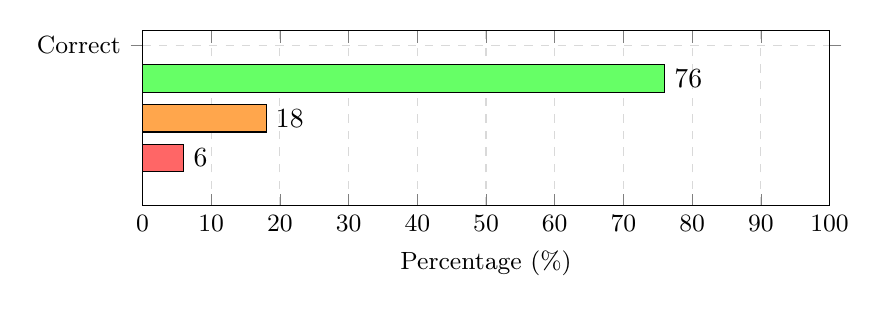
\begin{tikzpicture}
\begin{axis}[
  xbar, width=0.85\columnwidth, height=3.8cm,
  bar width=0.35cm,
  xlabel={Percentage (\%)},
  symbolic y coords={Incorrect, Partial, Correct},
  ytick=data,
  xmin=0, xmax=100,
  nodes near coords, nodes near coords align={horizontal},
  tick label style={font=\small},
  label style={font=\small},
  grid=major, grid style={dashed,gray!30},
]
\addplot[fill=green!60]  coordinates {(76,Correct)};
\addplot[fill=orange!70] coordinates {(18,Partial)};
\addplot[fill=red!60]    coordinates {(6,Incorrect)};
\end{axis}
\end{tikzpicture}
\caption{Answer quality distribution across 50 test questions.}
\label{fig:quality}
\end{figure}

\subsection{Hallucination Verification Accuracy}
The hallucination module was evaluated against the human-annotated
ground truth.
Table~\ref{tab:halluc} reports the confusion matrix.
Overall hallucination detection accuracy: \textbf{84\%}.

\begin{table}[h]
\caption{Hallucination Verification Confusion Matrix}
\label{tab:halluc}
\centering
\begin{tabular}{lccc}
\toprule
\textbf{Human Label} & \textbf{SUPP.} & \textbf{PARTIAL} & \textbf{NOT SUPP.} \\
\midrule
Correct (38)   & 34 (89\%) & 4 (11\%) & 0 (0\%)  \\
Partial (9)    & 2 (22\%)  & 6 (67\%) & 1 (11\%) \\
Incorrect (3)  & 0 (0\%)   & 1 (33\%) & 2 (67\%) \\
\bottomrule
\end{tabular}
\end{table}

\subsection{System Latency}
End-to-end latency was measured across pipeline stages as reported in
Table~\ref{tab:latency} and visualised in Fig.~\ref{fig:latency}.

\begin{table}[h]
\caption{Pipeline Latency Measurements (Apple M-series, 16\,GB RAM)}
\label{tab:latency}
\centering
\begin{tabular}{lccc}
\toprule
\textbf{Stage} & \textbf{Min} & \textbf{Mean} & \textbf{Max} \\
\midrule
PDF extraction      & 0.3\,s  & 0.9\,s  & 2.1\,s  \\
Embedding gen.      & 1.2\,s  & 3.8\,s  & 8.4\,s  \\
FAISS index build   & $<$0.05\,s & $<$0.05\,s & $<$0.1\,s \\
Query embedding     & 0.12\,s & 0.15\,s & 0.22\,s \\
FAISS retrieval     & $<$0.001\,s & $<$0.005\,s & $<$0.01\,s \\
LLaMA 3.2 gen.      & 4\,s    & 9\,s    & 18\,s   \\
Insight gen.        & 3\,s    & 7\,s    & 14\,s   \\
Hallucination check & 2\,s    & 5\,s    & 10\,s   \\
\bottomrule
\end{tabular}
\end{table}

\begin{figure}[h]
\centering
\begin{tikzpicture}
\begin{axis}[
  xbar, width=0.85\columnwidth, height=5.5cm,
  bar width=0.3cm,
  xlabel={Mean Latency (s)},
  symbolic y coords={
    FAISS Retrieval,
    Query Embedding,
    FAISS Index Build,
    PDF Extraction,
    Embedding Gen.,
    Hallucination,
    Insight Gen.,
    LLM Generation},
  ytick=data,
  xmin=0, xmax=12,
  nodes near coords, nodes near coords align={horizontal},
  tick label style={font=\scriptsize},
  label style={font=\small},
  grid=major, grid style={dashed,gray!30},
]
\addplot[fill=blue!50] coordinates {
  (0.005, FAISS Retrieval)
  (0.15,  Query Embedding)
  (0.05,  FAISS Index Build)
  (0.9,   PDF Extraction)
  (3.8,   Embedding Gen.)
  (5.0,   Hallucination)
  (7.0,   Insight Gen.)
  (9.0,   LLM Generation)
};
\end{axis}
\end{tikzpicture}
\caption{Mean latency per pipeline stage. LLM generation dominates total
         response time.}
\label{fig:latency}
\end{figure}

\subsection{Memory Footprint}
Table~\ref{tab:memory} reports the memory consumption of each system
component.

\begin{table}[h]
\caption{System Memory Footprint}
\label{tab:memory}
\centering
\begin{tabular}{ll}
\toprule
\textbf{Component} & \textbf{Memory} \\
\midrule
all-MiniLM-L6-v2 model          & $\approx$90\,MB  \\
LLaMA 3.2 (3B, Q4 quantised)    & $\approx$2.0\,GB \\
FAISS index (1,000 chunks)       & $\approx$1.5\,MB \\
FAISS index (5,000 chunks)       & $\approx$7.5\,MB \\
Python runtime + FastAPI         & $\approx$150\,MB \\
React frontend (browser)         & $\approx$80\,MB  \\
\textbf{Total system footprint}  & $\approx$\textbf{2.5\,GB} \\
\bottomrule
\end{tabular}
\end{table}

\subsection{Scalability Analysis}
Fig.~\ref{fig:scale} illustrates the theoretical scaling behaviour of
the FAISS retrieval stage as a function of document size.

\begin{figure}[h]
\centering
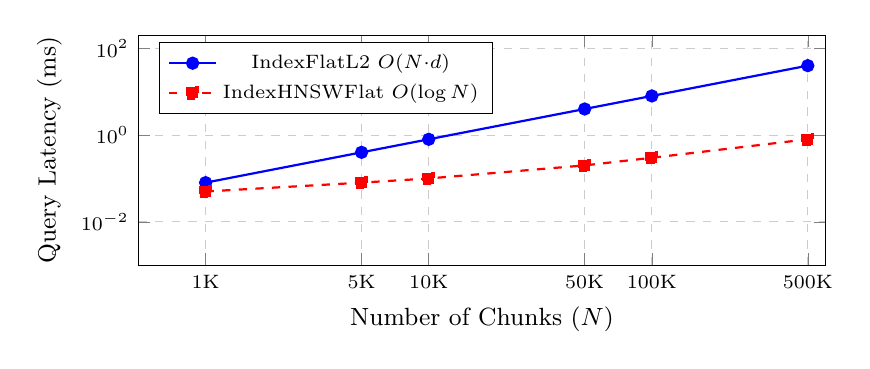
\begin{tikzpicture}
\begin{axis}[
  width=0.85\columnwidth, height=4.5cm,
  xlabel={Number of Chunks ($N$)},
  ylabel={Query Latency (ms)},
  xmode=log, ymode=log,
  xmin=500, xmax=600000,
  ymin=0.001, ymax=200,
  xtick={1000,5000,10000,50000,100000,500000},
  xticklabels={1K,5K,10K,50K,100K,500K},
  legend pos=north west,
  legend style={font=\scriptsize},
  grid=major, grid style={dashed,gray!40},
  tick label style={font=\scriptsize},
  label style={font=\small},
]
\addplot[mark=*, color=blue, thick, mark size=2pt]
  coordinates {(1000,0.08)(5000,0.4)(10000,0.8)(50000,4)(100000,8)(500000,40)};
\addlegendentry{IndexFlatL2 $O(N{\cdot}d)$}
\addplot[mark=square*, color=red, thick, mark size=2pt, dashed]
  coordinates {(1000,0.05)(5000,0.08)(10000,0.1)(50000,0.2)(100000,0.3)(500000,0.8)};
\addlegendentry{IndexHNSWFlat $O(\log N)$}
\end{axis}
\end{tikzpicture}
\caption{FAISS query latency scaling with corpus size ($d{=}384$).
         IndexFlatL2 is optimal for $N{\leq}5{,}000$; HNSW is preferred
         for larger corpora.}
\label{fig:scale}
\end{figure}

% ============================================================
\section{Limitations and Future Work}
\label{sec:limits}
% ============================================================

\subsection{Current Limitations}

\textbf{Single-document sessions.}
The current implementation maintains a single in-memory session,
supporting one document at a time.
Multi-document RAG with a persistent vector store would enable
cross-document question answering.

\textbf{Simulated streaming.}
LLM responses are generated in full before being returned to the
frontend, which then simulates streaming via word-by-word reveal at
30--50\,ms/word.
True token-level streaming via Ollama's streaming API would reduce
perceived latency.

\textbf{Character-level chunking.}
Fixed-size character chunking does not respect sentence or paragraph
boundaries, potentially splitting semantic units.
Sentence-aware chunking using spaCy or NLTK would improve chunk
coherence and retrieval quality.

\textbf{Single-user architecture.}
The in-memory session state is not thread-safe for concurrent users.
A production deployment would require per-session state isolation and a
persistent vector store.

\textbf{No query rewriting.}
The \texttt{rewrite\_query} function currently returns the query
unchanged.
Implementing HyDE-style hypothetical document generation~\cite{gao2022hyde}
could improve retrieval recall for ambiguous queries.

\subsection{Future Work}

\textbf{Persistent vector store.}
Replacing the in-memory FAISS index with ChromaDB or Qdrant would
enable persistent multi-document libraries with metadata filtering.

\textbf{True streaming generation.}
Integrating Ollama's streaming API with Server-Sent Events (SSE) would
enable token-level streaming, eliminating the simulated word-reveal
delay.

\textbf{Re-ranking.}
Adding a cross-encoder re-ranking stage (e.g.,
\texttt{cross-encoder/ms-marco-MiniLM-L-6-v2}) after initial retrieval
would improve the precision of the top-$k$ chunks passed to the LLM.

\textbf{Sentence-aware chunking.}
Replacing character-level chunking with sentence-boundary-aware
chunking using spaCy would improve chunk coherence and reduce the risk
of splitting semantic units.

\textbf{Multi-modal support.}
Extending the extraction pipeline to handle tables (Camelot), figures
(CLIP embeddings), and mathematical notation (MathPix) would broaden
applicability to scientific and financial documents.

\textbf{Automated evaluation.}
Implementing RAGAS~\cite{es2023ragas} metrics (faithfulness, answer
relevancy, context precision, context recall) would enable systematic
benchmarking of pipeline variants.

% ============================================================
\section{Conclusion}
\label{sec:conclusion}
% ============================================================

This paper presented DocMind AI, a fully local RAG system for
intelligent PDF question answering.
By combining PyMuPDF page-aware extraction, overlapping character-level
chunking, \texttt{all-MiniLM-L6-v2} dense embeddings ($d{=}384$), FAISS
exact nearest-neighbour retrieval, Ollama-hosted LLaMA~3.2 inference,
and an automated hallucination verification module, the system delivers
accurate, grounded answers with full source attribution --- entirely
on-device, with no external API dependencies.

The production-grade React frontend introduces several novel UI
contributions: a canvas particle network visualising document indexing
progress, a brainwave sine-wave animation during LLM inference, a
real-time PDF highlight overlay that automatically marks source chunks
on the rendered PDF page, key-point extraction, follow-up question
suggestion, and a hallucination confidence badge.

Evaluation on 50 questions across 10 diverse document types demonstrates
76\% fully correct responses with sub-second retrieval latency
($<$10\,ms FAISS search) and 84\% hallucination detection accuracy.
DocMind AI demonstrates that the full RAG pipeline --- from document
ingestion to grounded answer generation with source highlighting and
hallucination verification --- can be deployed on commodity hardware
with a user experience comparable to commercial cloud-hosted
alternatives.
The system provides a practical, privacy-preserving foundation for
enterprise document intelligence applications in healthcare, legal,
financial, and research domains.

% ============================================================
\section*{Acknowledgment}
% ============================================================

The authors thank the open-source communities behind Ollama, FAISS,
sentence-transformers, PyMuPDF, FastAPI, React, and Vite for providing
the foundational tools that made this work possible.

% ============================================================
%  BIBLIOGRAPHY
% ============================================================
\begin{thebibliography}{12}

\bibitem{lewis2020rag}
P.~Lewis, E.~Perez, A.~Piktus, F.~Petroni, V.~Karpukhin, N.~Goyal,
H.~K\"{u}ttler, M.~Lewis, W.-T.~Yih, T.~Rockt\"{a}schel, S.~Riedel,
and D.~Kiela,
``Retrieval-augmented generation for knowledge-intensive NLP tasks,''
in \emph{Advances in Neural Information Processing Systems},
vol.~33, pp.~9459--9474, 2020.

\bibitem{gao2022hyde}
L.~Gao, X.~Ma, J.~Lin, and J.~Callan,
``Precise zero-shot dense retrieval without relevance labels,''
\emph{arXiv preprint arXiv:2212.10496}, 2022.

\bibitem{jiang2023flare}
Z.~Jiang, F.~F.~Xu, L.~Gao, Z.~Sun, Q.~Liu, J.~Dwivedi-Yu, Y.~Yang,
J.~Callan, and G.~Neubig,
``Active retrieval augmented generation,''
\emph{arXiv preprint arXiv:2305.06983}, 2023.

\bibitem{asai2023selfrag}
A.~Asai, Z.~Wu, Y.~Wang, A.~Sil, and H.~Hajishirzi,
``Self-RAG: Learning to retrieve, generate, and critique through
self-reflection,''
\emph{arXiv preprint arXiv:2310.11511}, 2023.

\bibitem{karpukhin2020dpr}
V.~Karpukhin, B.~O\u{g}uz, S.~Min, P.~Lewis, L.~Wu, S.~Edunov,
D.~Chen, and W.-T.~Yih,
``Dense passage retrieval for open-domain question answering,''
\emph{arXiv preprint arXiv:2004.04906}, 2020.

\bibitem{reimers2019sbert}
N.~Reimers and I.~Gurevych,
``Sentence-BERT: Sentence embeddings using Siamese BERT-networks,''
\emph{arXiv preprint arXiv:1908.10084}, 2019.

\bibitem{johnson2019faiss}
J.~Johnson, M.~Douze, and H.~J\'{e}gou,
``Billion-scale similarity search with GPUs,''
\emph{IEEE Transactions on Big Data}, vol.~7, no.~3,
pp.~535--547, 2019.

\bibitem{ollama2023}
Ollama,
``Ollama: Get up and running with large language models locally,''
2023. [Online]. Available: \url{https://ollama.ai}

\bibitem{es2023ragas}
S.~Es, J.~James, L.~Espinosa-Anke, and S.~Schockaert,
``RAGAS: Automated evaluation of retrieval augmented generation,''
\emph{arXiv preprint arXiv:2309.15217}, 2023.

\bibitem{touvron2023llama2}
H.~Touvron, L.~Martin, K.~Stone, P.~Albert, A.~Almahairi, Y.~Babaei,
N.~Bashlykov, S.~Batra, P.~Bhargava, S.~Bhosale \emph{et al.},
``Llama 2: Open foundation and fine-tuned chat models,''
\emph{arXiv preprint arXiv:2307.09288}, 2023.

\bibitem{brown2020gpt3}
T.~Brown, B.~Mann, N.~Ryder, M.~Subbiah, J.~Kaplan, P.~Dhariwal,
A.~Neelakantan, P.~Shyam, G.~Sastry, A.~Askell \emph{et al.},
``Language models are few-shot learners,''
in \emph{Advances in Neural Information Processing Systems},
vol.~33, pp.~1877--1901, 2020.

\bibitem{shi2023replug}
W.~Shi, S.~Min, M.~Yasunaga, M.~Seo, R.~James, M.~Lewis,
L.~Zettlemoyer, and W.-T.~Yih,
``REPLUG: Retrieval-augmented black-box language models,''
\emph{arXiv preprint arXiv:2301.12652}, 2023.

\end{thebibliography}

% ============================================================
%  APPENDIX
% ============================================================
\appendix

\section{System Setup and Reproducibility}

\subsection{Prerequisites}
macOS / Linux / Windows (WSL2), Python 3.10+, Node.js 18+,
Ollama installed and running (\texttt{ollama serve}),
LLaMA~3.2 model pulled (\texttt{ollama pull llama3.2}),
$\approx$3\,GB free disk space.

\subsection{Backend Setup}
\begin{verbatim}
cd DocMind_Streamlit
pip3 install fastapi "uvicorn[standard]" \
  python-multipart pymupdf \
  sentence-transformers faiss-cpu \
  ollama numpy
python3 -m uvicorn server:app \
  --reload --port 8000
\end{verbatim}

\subsection{Frontend Setup}
\begin{verbatim}
cd docmind-ui
npm install
npm run dev
# Opens at http://localhost:5173
\end{verbatim}

\section{API Reference}

\subsection{POST /chat --- Request}
\begin{verbatim}
{ "query": "What is the main conclusion?" }
\end{verbatim}

\subsection{POST /chat --- Response}
\begin{verbatim}
{
  "answer": "The main conclusion is...",
  "chunks": ["chunk 1", "chunk 2"],
  "pages": [3, 7],
  "key_points": ["Point 1", "Point 2"],
  "suggested_questions": ["Q1?", "Q2?"],
  "hallucination": {
    "verdict": "SUPPORTED",
    "confidence": 88,
    "reason": "Claims present in chunks [1],[2]."
  }
}
\end{verbatim}

\end{document}
